\documentclass{article}
\title{CUDA Parallel Programming\\Homework 4}
\usepackage{graphicx}
\usepackage[UTF8]{ctex}
\usepackage{hyperref}
\usepackage{amsmath}
\CTEXoptions[today=old]
\author{40647007S 朱健愷}

\begin{document}
	\maketitle
	\section{Source codes}
	\subsection{File Layout}
	\begin{itemize}
		\item vecDotProduct\textunderscore{NGPU}/vecDotProduct\textunderscore{ngpu}.cu - First problem's main code used to calculate vector dot product that can utilize multi GPU
		\item headDiffusion2D\textunderscore{NGPU}/heatDiffusion2D\textunderscore{NGPU}.cu - Second problem's main code used to calculate heat diffusion in 2D grid using $\omega=1$
		\item Makefile - Script to auto generate executable from code
		\item vecDotProduct\textunderscore{NGPU}/experiment.sh - Script to auto generate results of first problem's vector dot product using multiple GPUs with different block size and grid size
		\item heatDiffusion\textunderscore{NGPU}/experiment.sh - Script to auto generate results of solving second problem's thermal 
		equilibrium temperature distribution on a square plate with different block size
		\item vecDotProduct\textunderscore{NGPU}/result/1GPU\textunderscore{block}\textunderscore*\textunderscore{grid}\textunderscore*/ - Output result of solving first problem's vector dot product with 1 GPU and different block size and grid size, the suffix represented the block size and grid size respectively. In this directory contains statistical result of calculating vector dot product.
		\item vecDotProduct\textunderscore{NGPU}/result/2GPU\textunderscore{block}\textunderscore*\textunderscore{grid}\textunderscore*/ - Output result of solving first problem's vector dot product with 2 GPU and different block size and grid size, the suffix represented the block size and grid size respectively. In this directory contains statistical result of calculating vector dot product.
		\item heatDiffusion2D\textunderscore{NGPU}/result/1GPU\textunderscore{block}\textunderscore* - Output result of solving second problem's 2D heat diffusion using 1 GPU and different block size, the suffix represent the block size. In this directory contains initial phi data, phi data calculated by GPU, and statistical result of solving 2D heat diffusion problem.
		\item heatDiffusion2D\textunderscore{NGPU}/result/2GPU\textunderscore{block}\textunderscore* - Output result of solving second problem's 2D heat diffusion using 2 GPU and different block size, the suffix represent the block size. In this directory contains initial phi data, phi data calculated by GPU, and statistical result of solving 2D heat diffusion problem.
		\item notebook/*.png - Plots concluding output result
	\end{itemize}
	
	
	\subsection{Usage}
	Make code in both vecDotProduct\textunderscore{NGPU}/ and heatDiffusion2D\textunderscore{NGPU}/ directories
	Run the experiment.sh script in both vecDotProduct\textunderscore{NGPU}/ and heatDiffusion2D\textunderscore{NGPU}/ directories 
	
	\begin{verbatim}
	cd vecDotProduct_NGPU
	make
	sh experiment.sh
	cd ../heatDiffusion2D_NGPU
	make
	sh experiment.sh
	\end{verbatim}
	
	And it will produce two problems statistical result using different block size and grid size.

	\subsection{Code design}
	In first problem, the program divide the vector into N equal portion of the original vector and use N GPU to calculate their dot product, and finally used CPU to gather N GPU's vector dot product result.
	
	In second problem, it divide the grid into $Nx\times{Ny}$ equal porition of the original grid and use $Nx\times{Ny}$ GPU to calculate the heat diffusion equation. While they are calculating the boundary, they will determine whether this is the true boundary which represent the edge of the plate or just the divided boundary that border to another portion of grid calculated by another GPU, and let CPU calculate the difference to determine whether it will perform the next grid update to minimize the error in consecutive iteration.

	\section{Result}
	\subsection{Experiment environment}
	I ran my code on workstation provided in course, below is the Setup of workstation
	\begin{itemize}
		\item Operating system: Linux version 4.19.172 (root@twcp1)\\(gcc version 6.3.0 20170516 (Debian 6.3.0-18+deb9u1))
		\item CPU: Intel(R) Core(TM) i7-4790 CPU @ 3.60GHz
		\item GPU: Nvidia GTX 1060 6GB
		\item Memory: 32GB 
	\end{itemize}
	\subsection{Performance}
	\subsubsection{First problem}
	Below four figures showed 1 GPU case and 2 GPU case performing dot product fixing one of block size or grid size and change the other one respectively
	\newpage
	\begin{figure}
		\centering
		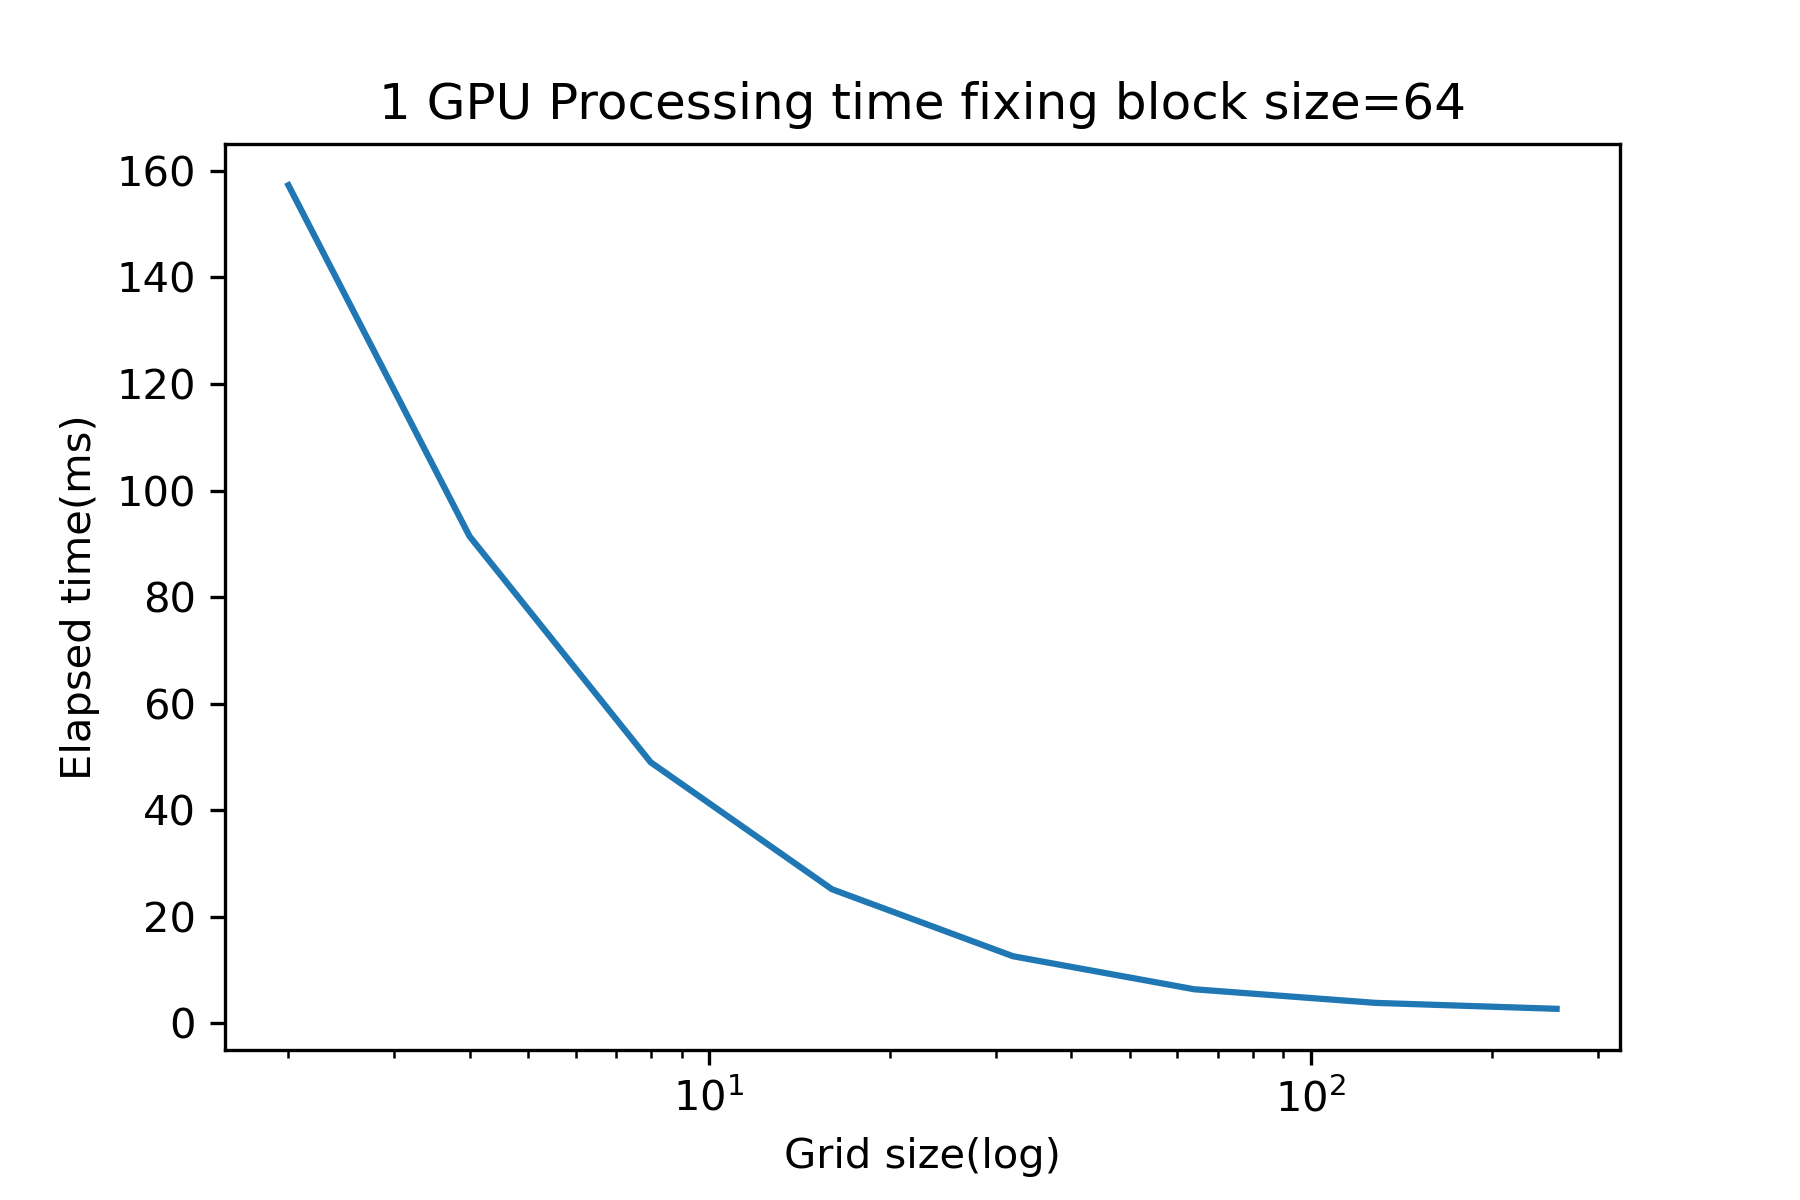
\includegraphics[width=\linewidth]{notebook/1gpu_processing_time_fix_block}
	\end{figure}
	\begin{figure}[hb!]
		\centering
		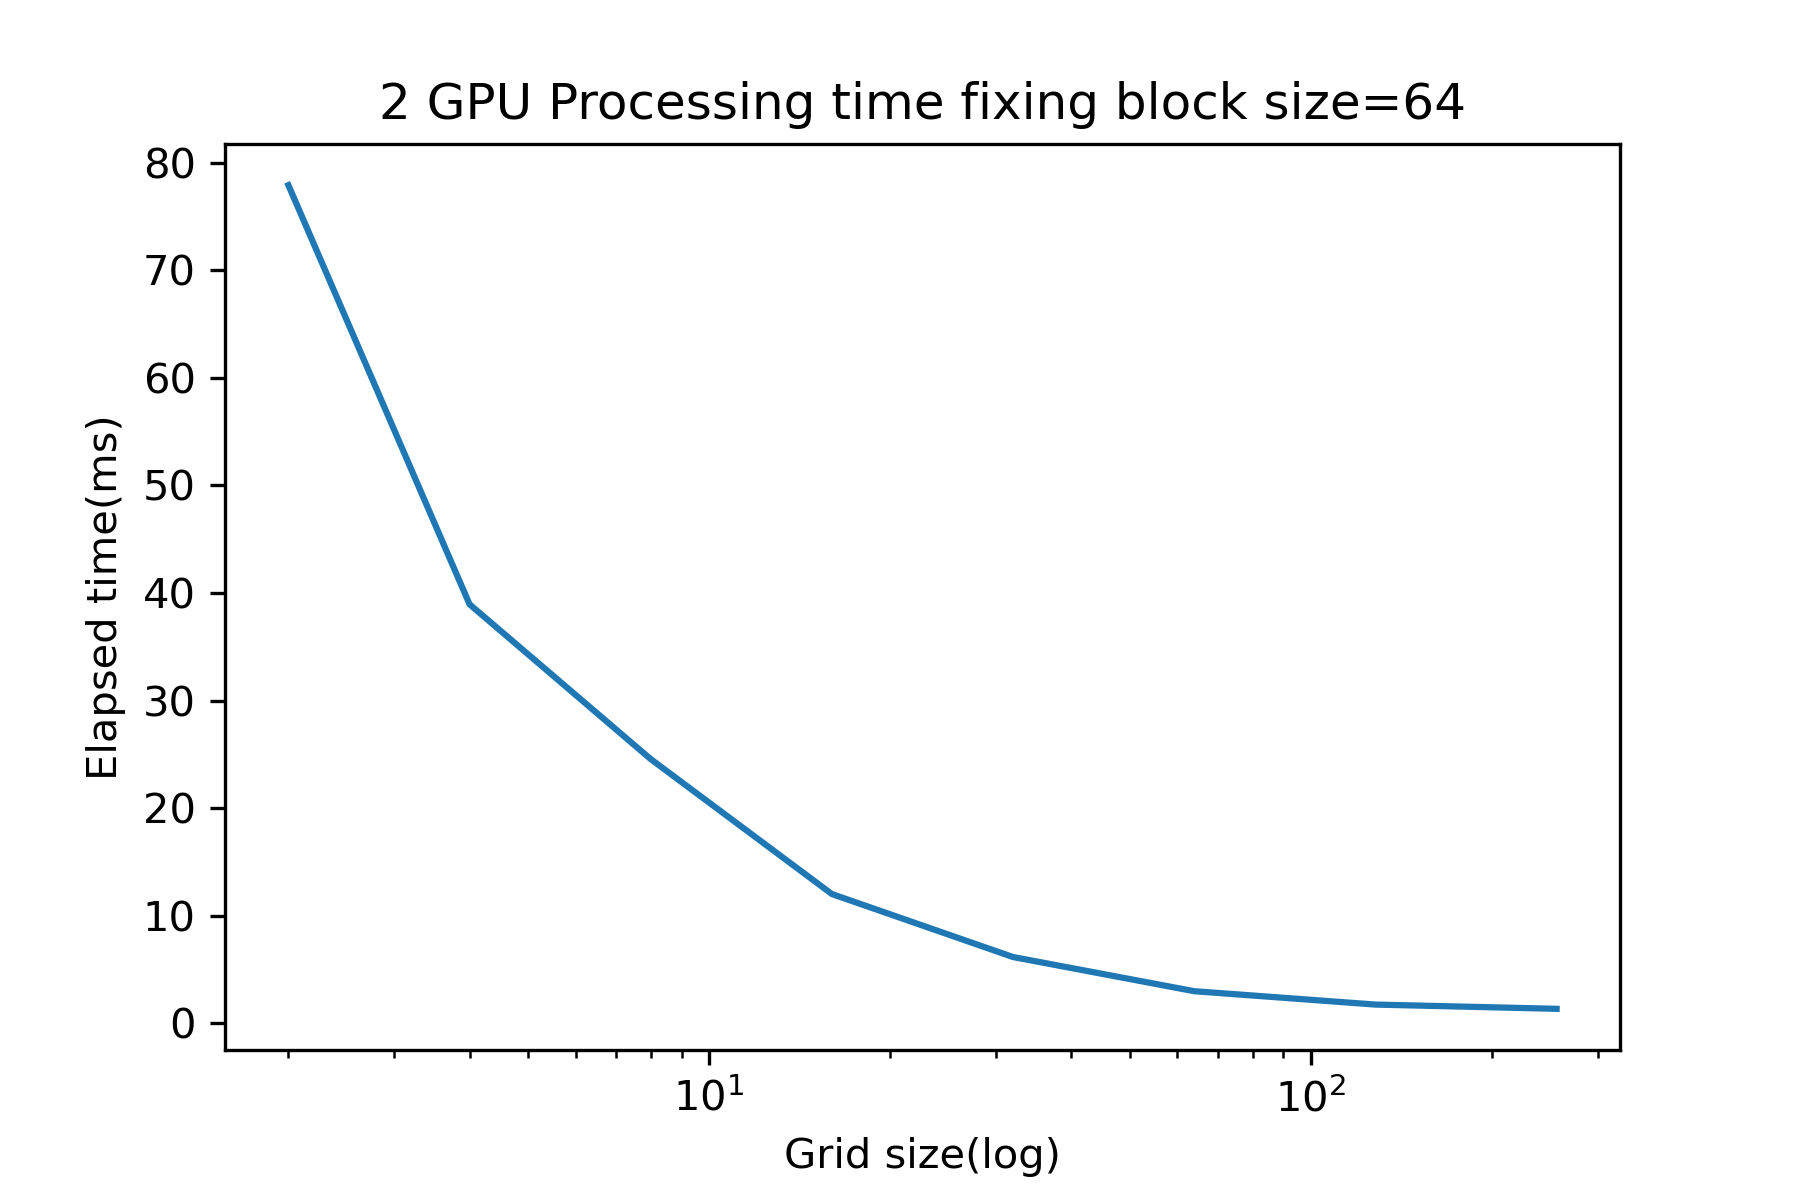
\includegraphics[width=\linewidth]{notebook/2gpu_processing_time_fix_block}
	\end{figure}
	\newpage
	\begin{figure}
		\centering
		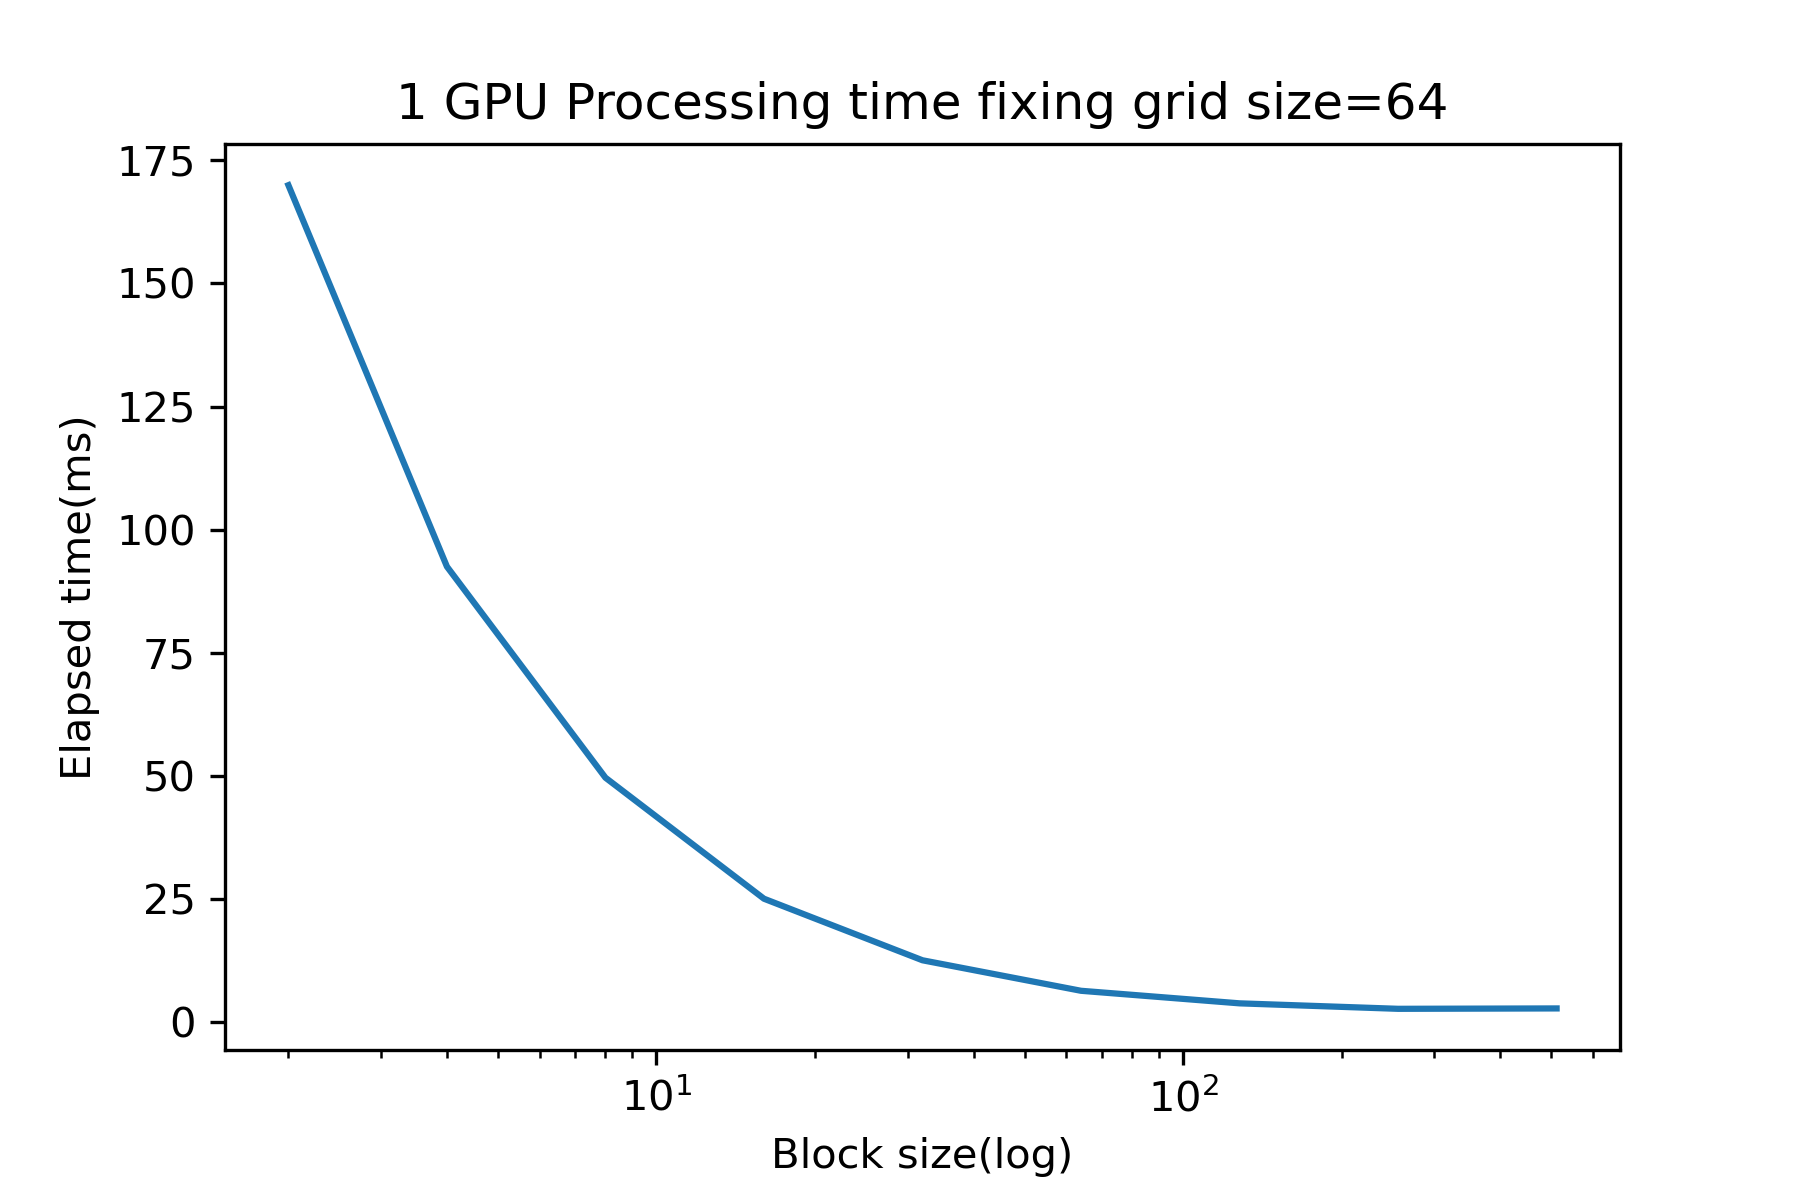
\includegraphics[width=\linewidth]{notebook/1gpu_processing_time_fix_grid}
	\end{figure}
	\begin{figure}[hb!]
		\centering
		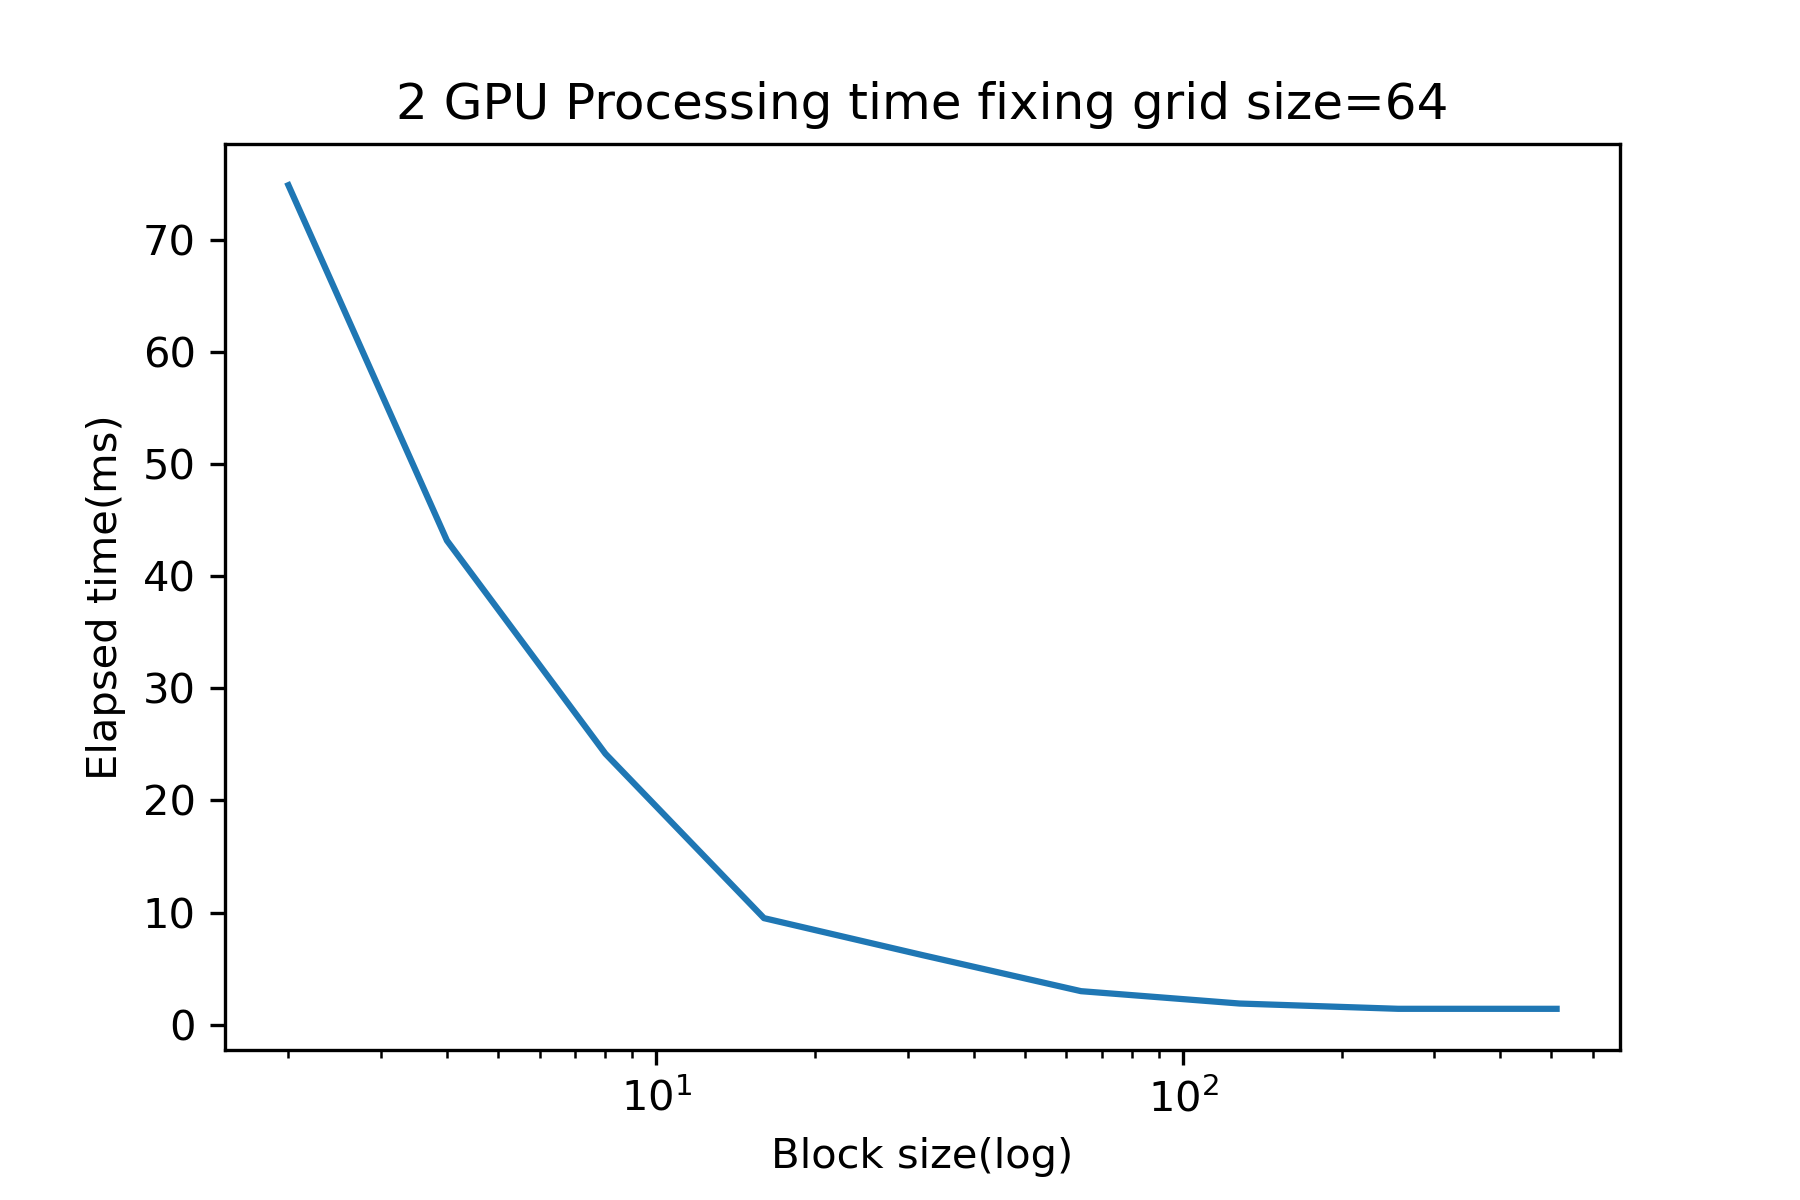
\includegraphics[width=\linewidth]{notebook/2gpu_processing_time_fix_grid}
	\end{figure}
	Below two figures showed 1 GPU case and 2 GPU case solving the 2D heat diffusion problem using different block size.
	\newpage
	\begin{figure}
		\centering
		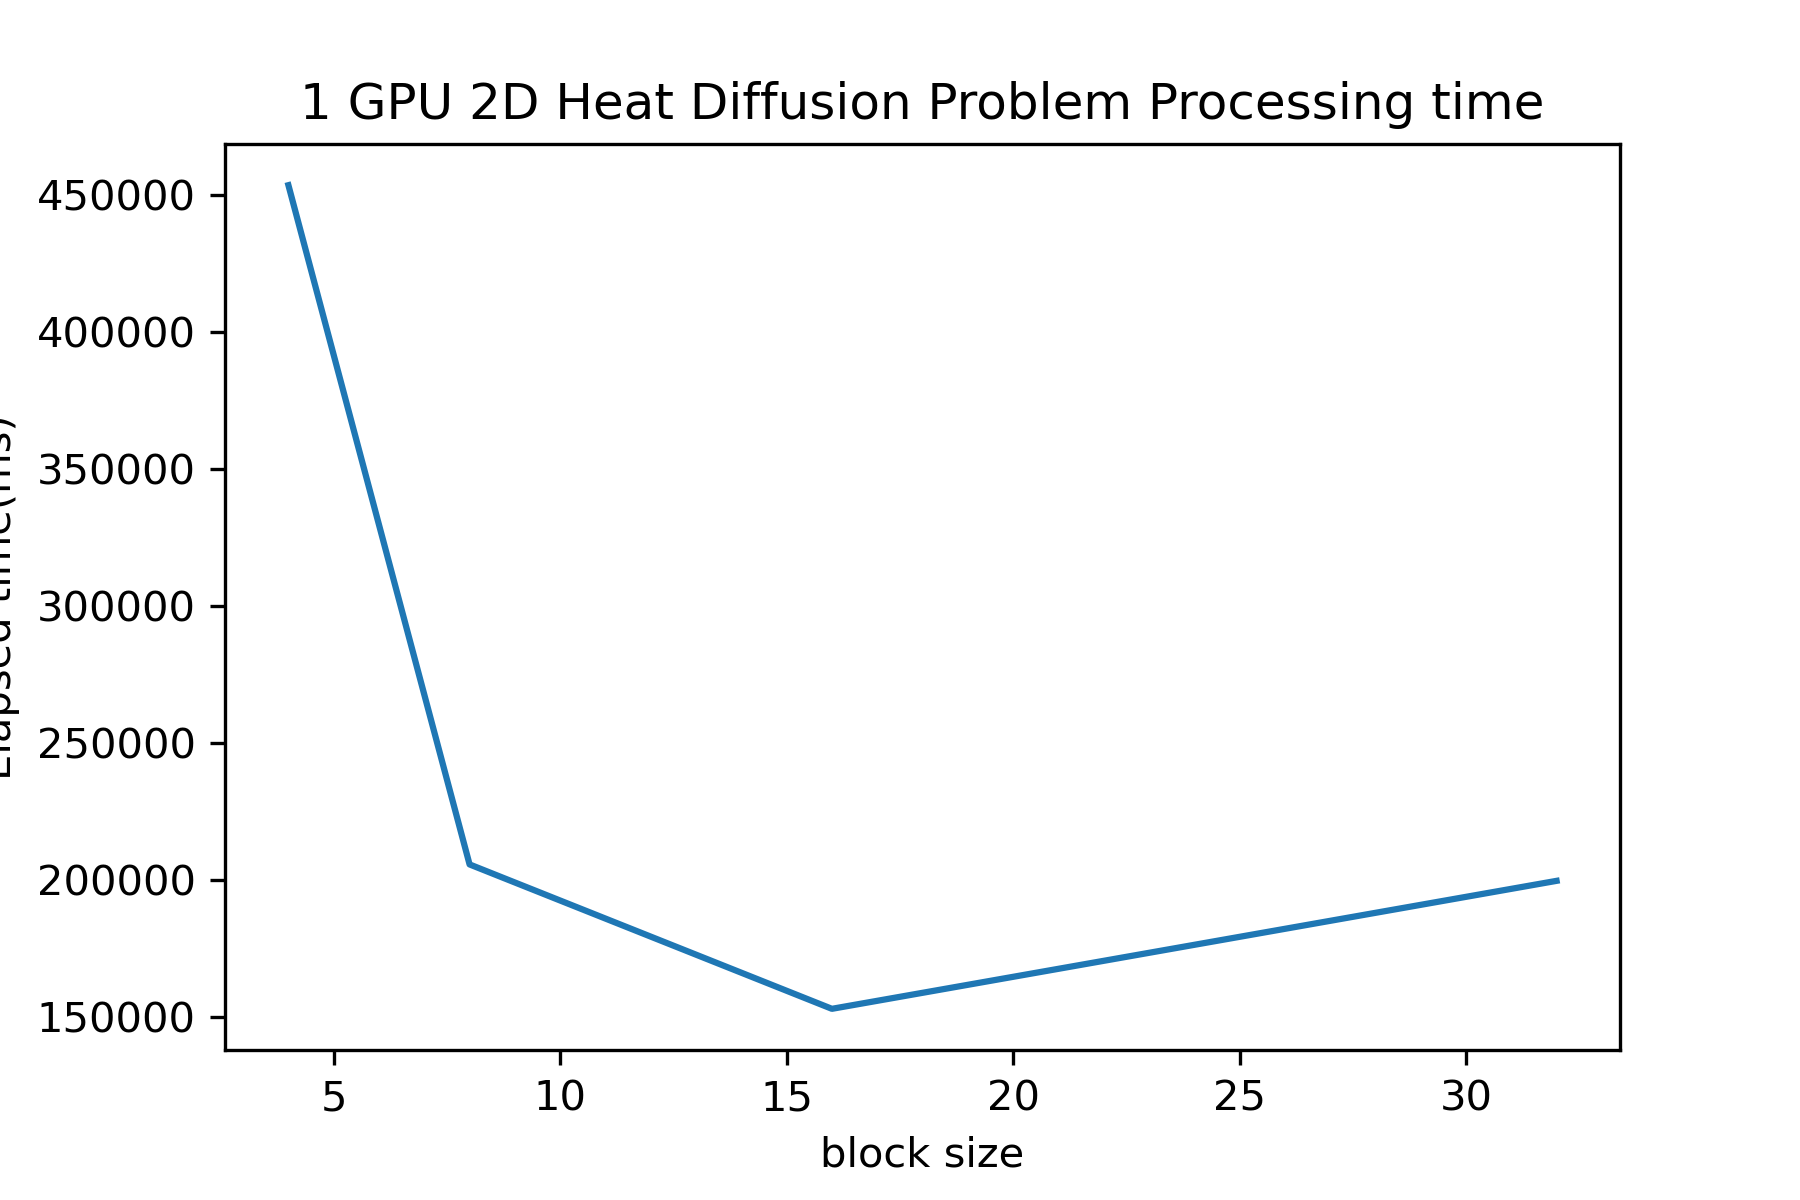
\includegraphics[width=\linewidth]{notebook/1gpu_heat_diffusion_processing_time}
	\end{figure}
	\begin{figure}[hb!]
		\centering
		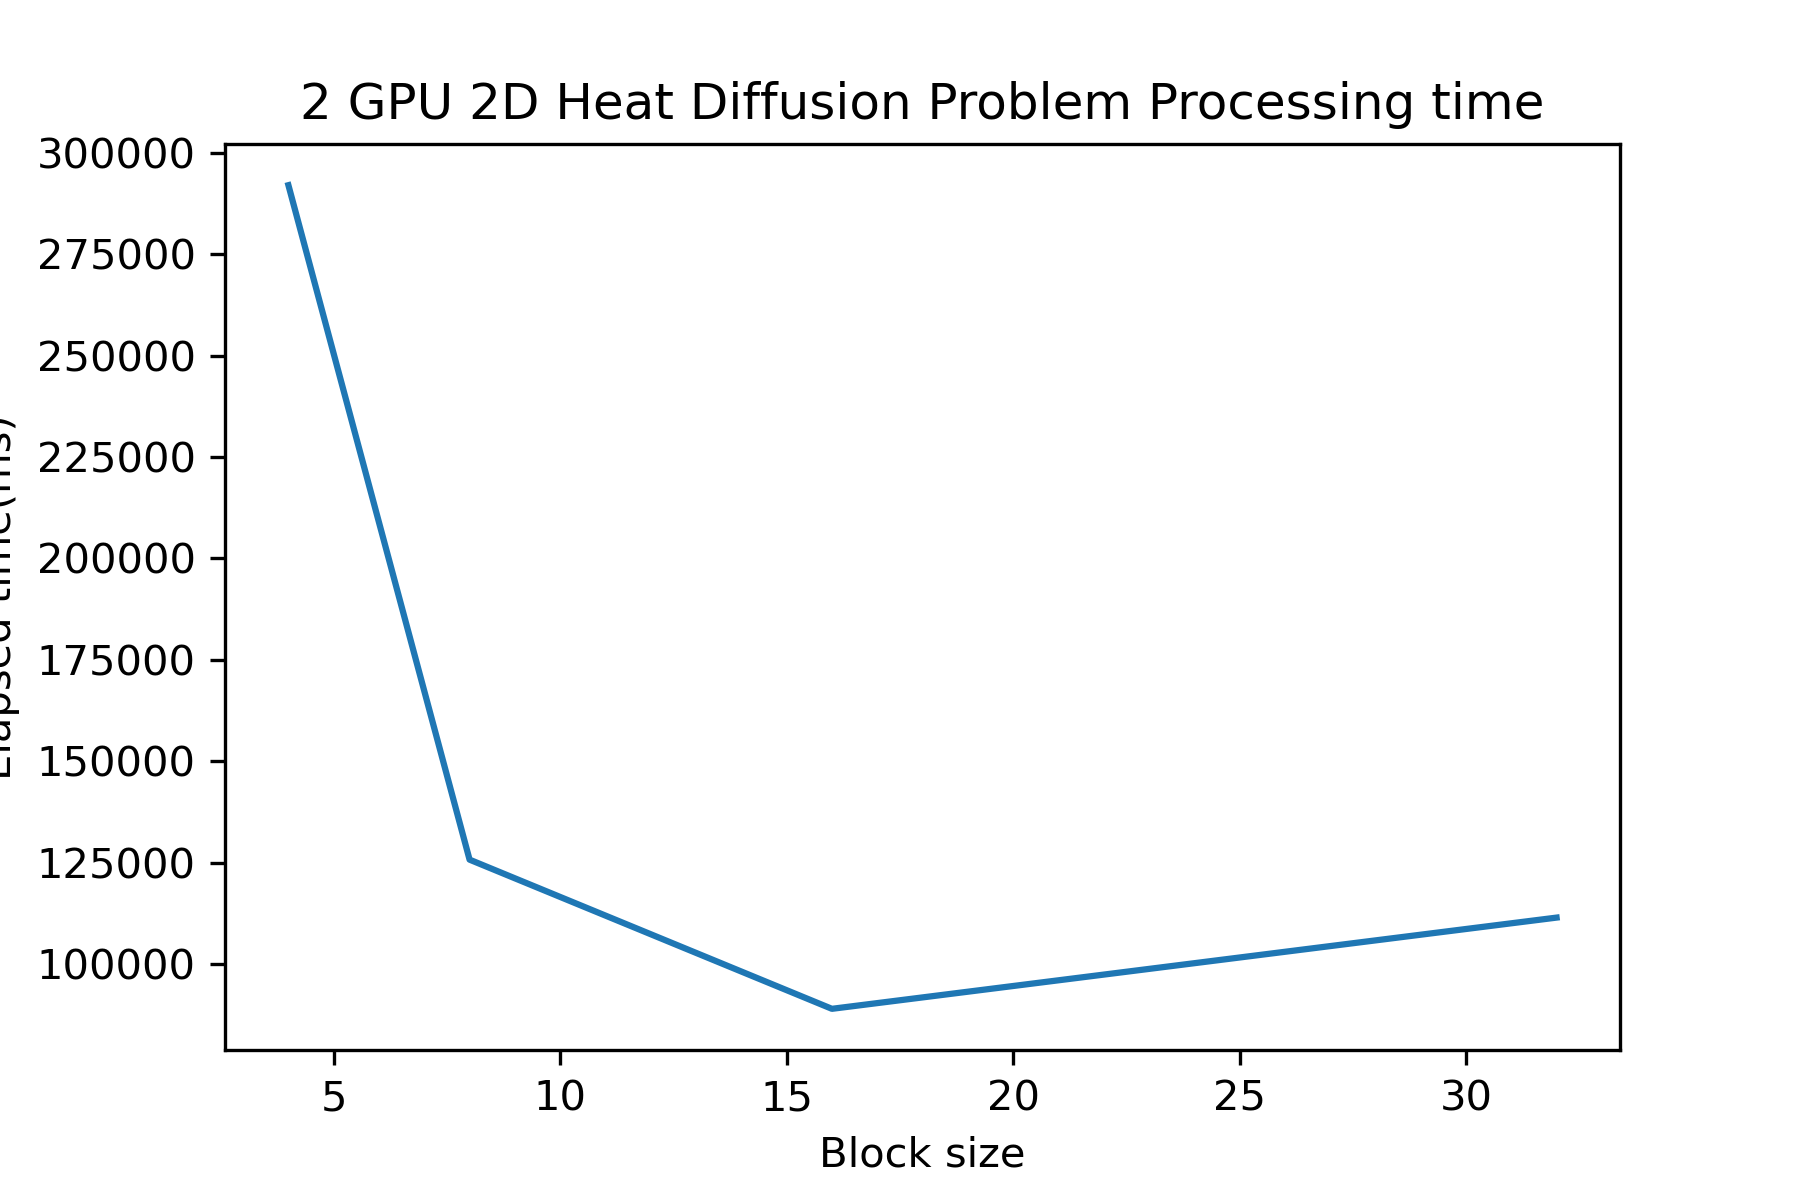
\includegraphics[width=\linewidth]{notebook/2gpu_heat_diffusion_processing_time}
	\end{figure}

	\subsubsection{Observation}
	We can observe that the performance of small block size setup in both 1 GPU case and 2 GPU case yield the worse performance in my experiment. This may because of when we do parallel reduction, we usually need many threads in block in order to collect each block's difference, and then gather the result using CPU, and more blocks in grid in order to collect dot product data which range are out of basic per threads in grid. So the block size and grid size do affect the performance a lot.
	
	The result of utilizing 2 GPU in both problems helps improve the performance in nearly every block size and grid size setup(except for very large grid or block size setup), in my observation, they spent nearly half times of calculation time as 1 GPU cases in both problem. But same as the observation I observed in the previous assignment, the performance increase until block size or grid size increased to some extent. 
	
	The optimal block size and grid size setup for first problem in my experiment is 256 block size and 256 grid size for 1 GPU case, 256 block size and 64 grid size for 2 GPU case.
	
	The optimal block size setup for second problem in my experiment is 16 block size for 1 GPU case and 16 block size for 2 GPU case.
	
	\section{Discussion}
	I thought their speed up is due to divide the question into two equal portion and solve them. So we can see the approximately one times speed up compared to 1 GPU case in both problem. Although the second problem demanded that 2 GPU have to communicate between boundary to solve the problem, that's not the bottleneck, because in this two problem, synchronizing between 2 GPU, 4 GPU or even more GPU requires fix GPU bridge amount(In first problem 0 bridge is required, in second problem up to 4 bridges for each GPU is required), unless the problem scale is arbitrary large or too many GPU to synchronize that had filled the GPU bandwidth of transferring data.
\end{document}